\section{Computational cost}
\label{sec:performance}
% P:performance-01
The cost of a request depends on what it returns, so cost is compared by operation and only where two codes return the same values.
Five operations are distinguished (Table~\ref{tab:cost}): a property bundle of a state at fixed density; a state at fixed pressure, which adds density closure; a declared equilibrium solve; an explicit phase discovery; and first-order actions on a state that is already solved.
FeOs~0.10.1~\citep{rehnerFeOsOpenSourceFramework2023} and Clapeyron.jl~0.6.29 under Julia~1.13.1~\citep{walkerClapeyronjlExtensibleOpenSource2022} supply the comparator implementations.
A timing comparison requires scaled property differences below $10^{-8}$, relative density-closure differences below $10^{-10}$, relative equilibrium pressure and density differences below $10^{-7}$, and absolute composition and phase-fraction differences below $10^{-8}$.
Every timed comparator case met these criteria.
Initial model construction, process startup, Julia compilation, warmups and request transport are excluded.
The central-difference timings include constructing shifted parameter records and mixtures and re-solving the displaced states.
Each code runs in its own persistent worker process, and two independent package workers bracket the FeOs and Clapeyron.jl workers in alternating order over three repetitions.
Each worker's time is the median of its three block medians of warm calls.
Each paired ratio divides a package block median by the comparator block median from the same repetition; the reported ratio is the median of the six such ratios, two package workers by three repetitions, with their full range beside it.
That range describes observed spread, not a confidence interval.
The ratios compare the calls each code exposes for the same result, not equal algorithms, and they hold for one host.

% P:performance-02
The marginal cost of exact derivatives is reported as actions on a solved state: the time of the first-order actions after a central solve, against the time of central differences that re-solve the state at shifted inputs.
The ethanol--butane bubble-point actions return pressure and vapor composition along temperature, the binary interaction parameter and the two ethanol association parameters; the water--pentanol actions return the water mole fraction of each liquid and the water-rich phase amount along temperature and the binary interaction parameter.
That ratio excludes the central solve, which both routes need, so it is not a speedup of a whole calculation or a comparison with another code's implicit derivatives.
No comparator was timed on charged or reacting cases, and no comparative cost claim is made for them.

% P:performance-03
The fixed-density bundle uses propane at 300~K and 500~mol\,m$^{-3}$; density closure uses a changing-pressure sequence of liquid propane states at 300~K near 1.9974~MPa.
Declared equilibrium cases are propane saturation at 300~K, equimolar ethanol--butane bubble pressure at 373.15~K, and an equimolar water--pentanol liquid split at 298.15~K and 101.3~kPa.
Explicit discovery uses equimolar methane--ethane at 190~K and 1~MPa, a two-phase point at which all three codes return the same phases.
At another methane--ethane point the codes did not return the same state quantities, so that point was not timed and the discovery ratio does not extend to other points.
Measurements used an AMD Ryzen 9 5900XT with 32 logical CPUs, workers pinned to logical CPU~31 with one numerical thread each, and one-minute load averages of 3.37--3.95 before and after the selected blocks; a block was admitted only when the load average was below 4 before and after it.
Each worker supplied 75 samples for each property-bundle and declared-equilibrium case, 15 for density closure and discovery, and 30 for each exact-action or central-difference set, across three blocks.
The electrolyte calculation was timed for the package only: the eight water/ethanol/isobutanol/NaCl feeds of Section~\ref{sec:cross-code} (Fig.~\ref{fig:electrolyte-lle}a) at 293.15~K and 100~kPa with constant permittivity, with 15 samples per worker.
The first package worker's median was 154.6~ms for the whole eight-feed set, with block medians from 154.6 to 156.6~ms; the second package worker gave 160.5~ms, from 158.5 to 164.4~ms.
One propane-saturation block exceeded the load-average limit, so it was excluded and the complete saturation operation was repeated with all workers; the selected measurements contain 102 blocks and 1590 samples.

\begin{table}[pos=htbp]
\centering
\caption{Package time divided by comparator time for value-matched operations, and exact-action time divided by the package's central-difference time on the same solved state: median [minimum, maximum] of six paired block ratios.
Values below unity mean less package or exact-action time; the density-closure comparison with Clapeyron.jl is a tie within the observed spread.}
\label{tab:cost}
\small
\begin{tabularx}{\linewidth}{@{}Xcc@{}}
\toprule
Operation and case & Package / FeOs & Package / Clapeyron.jl \\
\midrule
Property bundle at fixed density, propane & 0.2147 [0.0690, 0.2346] & 0.5058 [0.4370, 0.8999] \\
Density closure at fixed pressure, liquid propane & 0.2728 [0.2447, 0.4857] & 0.8457 [0.5677, 1.469] \\
Declared equilibrium: propane saturation & 7.260 [5.726, 7.524] & 4.514 [4.091, 5.229] \\
Declared equilibrium: ethanol--butane bubble point & 1.940 [1.883, 2.106] & 0.8189 [0.7067, 0.8714] \\
Declared equilibrium: water--pentanol liquid--liquid split & 0.2841 [0.2828, 0.2897] & 1.957 [1.492, 2.018] \\
Explicit phase discovery: methane--ethane & 32.50 [30.14, 32.84] & 11.76 [10.40, 15.89] \\
\midrule
\multicolumn{3}{@{}l}{Exact first-order actions / package central differences, central solve excluded} \\
Ethanol--butane bubble point & \multicolumn{2}{c}{0.02766 [0.02654, 0.05074]} \\
Water--pentanol liquid--liquid split & \multicolumn{2}{c}{0.009577 [0.008246, 0.01233]} \\
\bottomrule
\end{tabularx}
\end{table}

% P:performance-04
The property bundle costs less than either comparator, and density closure costs less than in FeOs and ties with Clapeyron.jl within the observed spread (Fig.~\ref{fig:cost}).
For the ethanol--butane bubble point and the water--pentanol split the package time lies between the two comparator times, whereas propane saturation takes 4.5 and 7.3 times and explicit discovery 11.8 and 32.5 times the Clapeyron.jl and FeOs times.
These measurements do not isolate the causes: the codes differ in initialization, reuse of previous results, stopping rules and discovery method, and matching the returned state does not establish equivalent phase-search coverage or a package-wide speed factor.
The two solved-state action ratios quantify marginal derivative cost only.

\begin{figure}[pos=htbp]
\centering
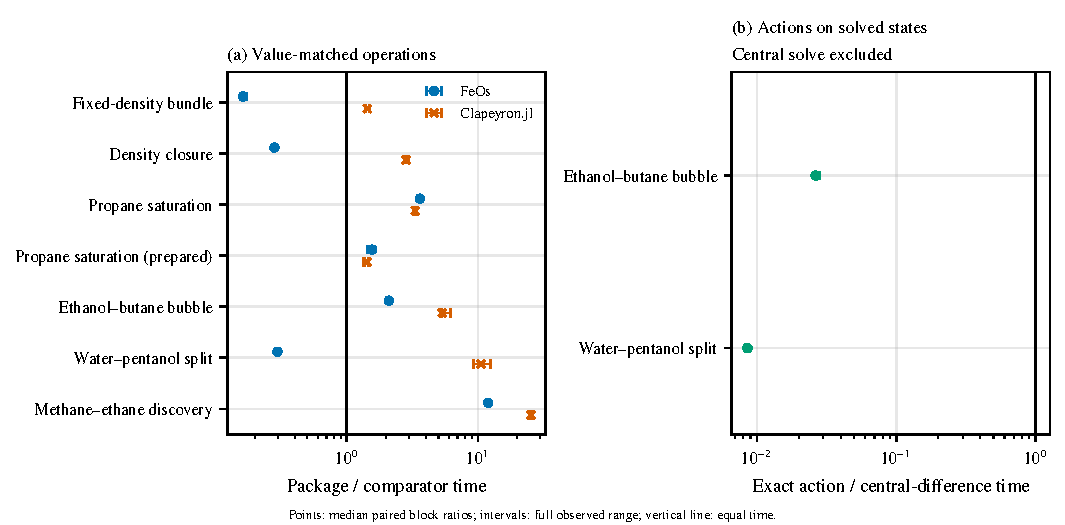
\includegraphics[width=\linewidth]{F6-computational-cost}
\caption{Value-matched computational costs.
(a) Package time over FeOs or Clapeyron.jl time for each operation; the fixed-density bundle and density closure use propane.
(b) Exact first-order action time over the package's central-difference time on an already solved state, excluding the central solve.
Points show medians and horizontal intervals the full ranges of six paired block ratios; the vertical line marks equal time, and points left of it mean less package time in (a) and less exact-action time in (b).
The electrolyte calculation has no comparator and is excluded.}
\label{fig:cost}
\end{figure}
\clearpage
